\begin{figure}[!htb]
    \begin{center}
    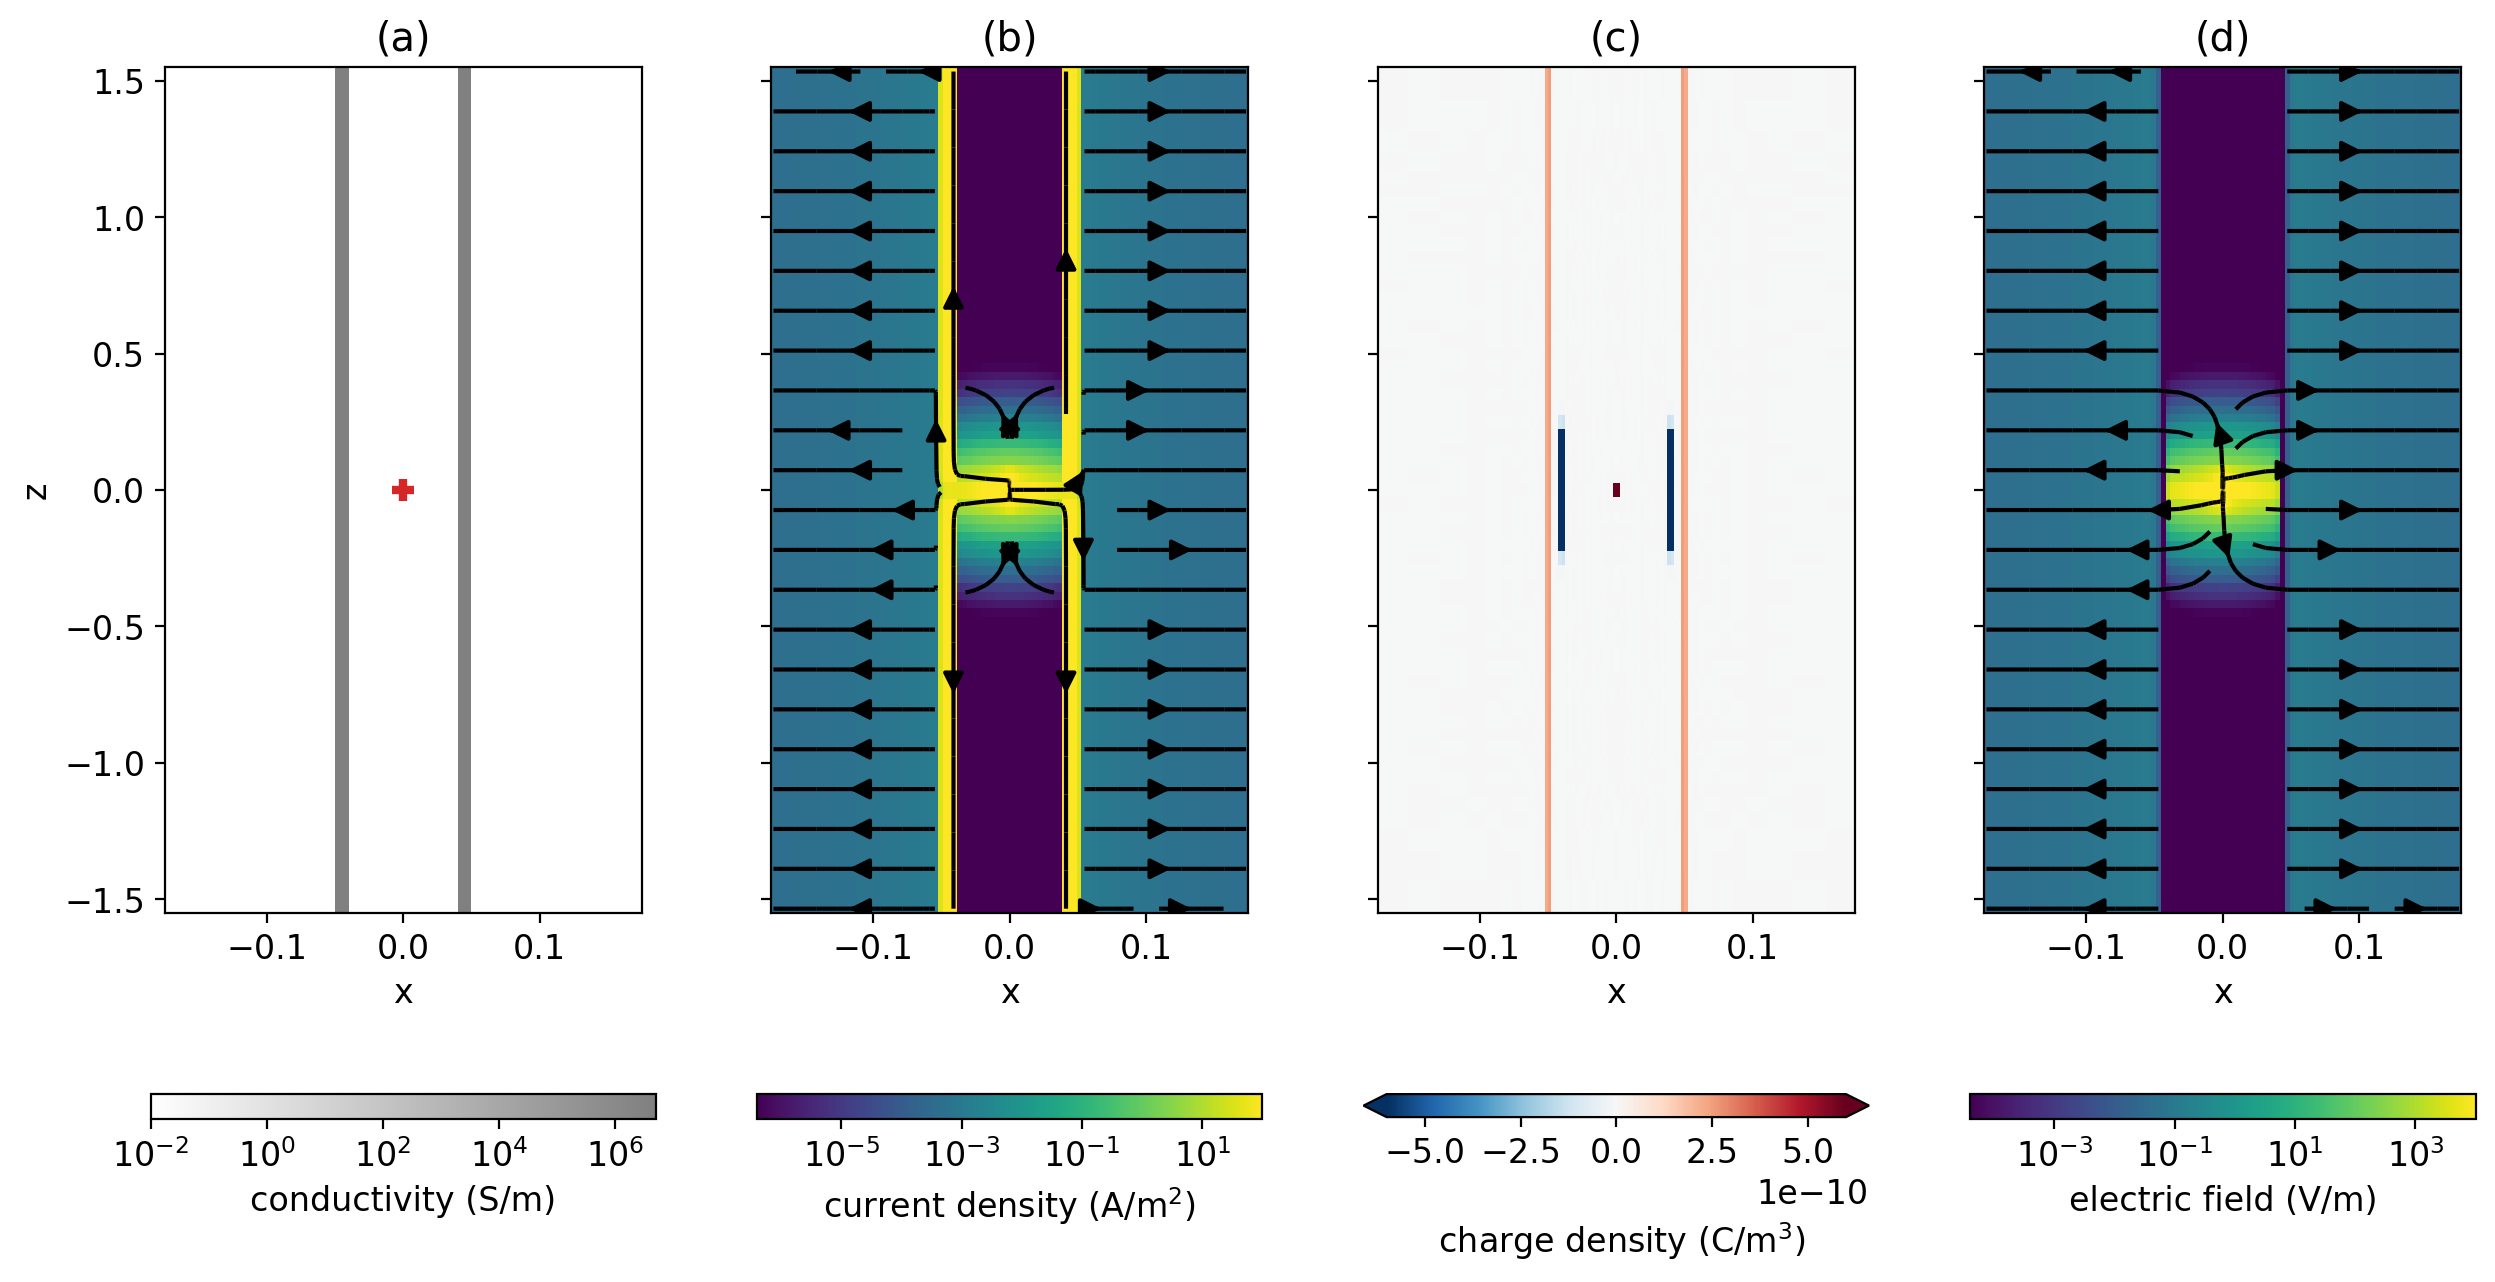
\includegraphics[width=0.9\textwidth]{figures/kaufman-dc.png}
    \end{center}
\caption{
    DC resistivity experiment where a point source is positioned inside of a long steel-cased well $5\times10^6$ S/m in a $100$ $\Omega$m wholespace. (a) Conductivity model with positive electrode location (red plus); (b) current density; (c) charge density, note that the colorbar has been saturated; (d) electric fields. Figure follows \cite{Heagy2019a}
}
\label{fig:kaufman-dc}
\end{figure}
